\documentclass[11pt, a4paper]{article}

\usepackage{tikz}
\usepackage{amsmath}
\usepackage{amsfonts}
\usepackage{mathtools}
\usepackage{graphicx}
\usepackage{multicol}
\usepackage{appendix}
\usepackage{pgfplots}
\usepackage{algorithm}
\usepackage{algpseudocode}
\usepackage[utf8]{inputenc}
\usepackage[english]{babel}

\pgfplotsset{compat=1.16}

\date{}
\title{Exoplanets detection using \\ Auto-Tuned Random Forest}

\author{Lorenzo Loconte \\ \small Knowledge Engineering Project \\ \small University of Bari Aldo Moro, Department of Informatics}

\begin{document}

\maketitle
\begin{abstract}
  The \texttt{NASA Kepler} project consists of discovering exoplanets (i.e. planets outside our solar system).
  The data generated by the \texttt{Kepler Space Telescope} is analyzed by humans and algorithms to discover new exoplanets.
  The main problem is that a lot of exoplanets are revealed false positives.
  This work consists of identifying exoplanets using random forest, a \textit{Supervised Machine Learning} model.
  Furthermore, the fitted model is analyzed in order to determine which features are relevant.
  The hyperparameters are automatically optimized with techniques that come from the \texttt{AutoML} research.
  In fact, the hyperparameters of the model are optimized and cross-validated with \texttt{Hyperband}, a simple yet effective and scalable method for hyperparameters optimization.
\end{abstract}

\clearpage

\section{Introduction}
  \paragraph{Kepler Object of Interest}
    Exoplanets are particular planets that are situated outside our solar system which orbit around one star (sometimes even multiple stars).
    The \texttt{NASA Kepler} project aims to discover these objects by looking at some stars and observing their luminosity during time.
    Basically suppose we are observing a star.
    If a rapid decrease and consequently increase of its luminosity occurs it's most likely that an object passed the way between us and the star.
    Analyzing the variation of luminosity for a certain amount of time we can extrapolate features like the radius and the orbit eccentricity of the object.
    Sometimes these object are actually exoplanets but it's common they can be something else like asteroids or even another star.
    Sometimes they are just false positives due to measurements noise.

    The goal of this work is to build a model (using \textit{Supervised Machine Learning}) that is capable to determinate if a hypothetical exoplanet can be confirmed or is just false positive.
    The dataset used is the cumulative list of \texttt{Kepler Object of Interest} (\texttt{KOI}) tables that come from the \texttt{NASA Kepler} project of discovering exoplanets.
    The complete dataset can be found at \texttt{https://exoplanetarchive.ipac.caltech.edu}.
    The dataset is composed by a list of hypothetical exoplanets.
    Each sample have a label indicating if the corresponding exoplanet is candidate, false positive or confirmed.
    The provided dataset consists of a lot of heterogeneous features.
    For the classification task the selected features can be found in Appendix \ref{appendix:features}.
    
    The candidate exoplanets (i.e. the exoplanets which existence is uncertain) are discarded in order to reduce noise and improve the learning process.
    For simplicity all the samples having null values are discarded from the dataset.
    Furthermore, all the selected features are numeric and the preprocessing method applied to the dataset is the standard normalization.
    The resulting dataset contains \texttt{5860} samples, of which only \textasciitilde \texttt{38\%} are confirmed and the remaining are false positives.

  \paragraph{Random Forests}
    As described before, the classification task consists to determinate if some numerical characteristics can be attributed to an existing exoplanet.
    The model used for the classification task is a random forest, a bagging ensemble of decision trees.
    The prediction of the random forest is computed as the mode of the predictions made by the decision trees.
    Note that each tree of the forest is trained on a subset of the features.
    Random forests correct the habit of decision trees of overfitting on their training set.
    In fact, decision trees tend to overfit their training sets because they have a low bias but an high variance.

    In \textit{Supervised Machine Learning}, bias consists of erroneous assumptions about the data and variance is a measure of sensitivity to the noise in the training data.
    So, random forests generally obtain better performance.

    The law that regulates the bias and variance is called \texttt{Bias-Variance tradeoff} \cite{biasvariance}.
    This law states that models having low bias have an high variance and vice versa.
    In \textit{Machine Learning} bias and variance corresponds to the models behaviors that we want to regulate in order to minimize the error.
    An high bias causes \textit{underfitting} while an high variance causes \textit{overfitting}.
      \[\mathrm{Error}=\mathrm{Bias}^{2}+\mathrm{Variance}+\mathrm{Irreducible\:Error}\]

  \paragraph{Hyperparameters}
    Often it's difficult (or nearly impossible) to select the correct hyperparameters that guarantee good performance on some specific datasets.
    \texttt{AutoML} is a branch of \textit{Machine Learning} that try to simplify the process of model selection and hyperparameters optimization.
    This work focuses on solving the hyperparameters search problem for random forests.
    The algorithm used is \texttt{Hyperband} that, as it'll be shown in the next section, represents an evolution of random search designed especially for hyperparameters optimization.

    For the hyperparameters optimization algorithm chosen, the number of trees in the random forest is not considered an hyperparameter.
    Furthermore, the following hyperparameters are optimized:
    \begin{itemize}
      \item The split criterion (Gini Impurity or Information Gain, see Appendix \ref{appendix:splitcriterions} for details)
      \item The fraction of features to use for each tree
      \item The fraction of samples used to train each tree
      \item The maximum depth of each tree
      \item The minimum number of samples required to split an internal node
      \item The minimum number of samples to be at a leaf node
    \end{itemize}

\clearpage

\section{Hyperparameters Optimization}
  In this section it will be shown a formalization of the hyperparameters optimization task as a search problem.
  In this work we refer to hyperparameters as the ones that cannot be trained (e.g. the ones described in the previous section).
  After that we briefly introduce the hyperparameters optimizer used in this work, \texttt{Hyperband}, as described in \cite{hyperband}.

  Given a training set $T$, a model $L$ and its hyperparameters search space $\Omega$, the hyperparameters optimization task consists to find an hyperparameters configuration $\omega \in \Omega$ such that the resulting model $L\langle\omega\rangle$ maximizes a certain score $S$ using cross-validation on $T$.
  Note that most search algorithms don't converge to the global maximum.
  So, the goodness of the hyperparameters found is dependent of the amount of resources we have.

  There are a lot of different techniques for hyperparameters optimization, some of them are the following:
  \begin{itemize}
    \item Random Search
    \item Grid Search
    \item Hyperband
    \item Bayesian Optimization
    \item Hybrid Approaches (like \texttt{BOHB} \cite{bohb})
  \end{itemize}

  Of the techniques cited above only \texttt{Bayesian Optimization} guarantees the convergence to the global maximum in the hyperparameters search space (see \cite{bayesianoptimization} for details).
  The simplest algorithm is \texttt{Random Search} and it works well if the hyperparameters search space is not too big.
  \texttt{Random Search} is expensive because each evaluation of the score function is done on models completely built from scratch.
  So, each evaluation of the score function on some randomly selected hyperparameters will use the same amount of computational resources, even if some hyperparameters of the search space obtain a very low score.
  The idea behind \texttt{Hyperband} is that it's better to save up resources on these hyperparameters configurations that doesn't obtain a sufficiently good score by gradually building more complex models over time.
  
  Note that we refer to budget as the computational cost of cross-validating a certain model.
  For example, for neural networks the budget can be the number of training epochs, while for random forests it can be the number of trees.

  Algorithm \ref{algorithm:hyperband} shows an implementation of \texttt{Hyperband} as described now.
  Given a budget $R$, \texttt{Hyperband} consists of random sampling some points (for example using the uniform distribution) in the hyperparameters space and cross-validating them using only a fraction of the budget $R$.

  After that we pick a fraction $1/\eta$ of the best models.
  In this way we discard the models that didn't obtain a sufficiently good score saving up computational resources.

  After that, we strengthen the previous models using a larger portion of $R$ and iterate in this way until we use the complete budget $R$.
  The procedure of consequently eliminating hyperparameters samples that don't obtain a good score is called \texttt{Successive Halving}.
  The fraction of the budget to use for each iteration grows geometrically in respect of $\eta$.
  Furthermore, we execute the discussed algorithm multiple times using less and less initial random points and using an higher starting budget.
  So, initially \textit{exploration} is preferred and \textit{exploitation} is performed later.

  Even if \texttt{Hyperband} is a simple algorithm, it is well scalable on multiple CPUs because we assume that every point in the hyperparameters space is independent from the others.

  In our case the model $L$ is a random forest.
  As said before, the budget $R$ is the maximum number of trees that the final random forest will have.
  The choice of the score $S$ is dependent from the task.
  For simplicity the $F_{1}$ score is used (i.e. we want to maximize both \textit{Precision} and \textit{Recall}).
  In this work the hyperparameters search space can be defined formally as:
  \[\Omega = \overbrace{\{gini, entropy\}}^{\text{Split criterion}} \quad\times \overbrace{(0, 1]}^{\text{Features fraction}} \times \overbrace{(0, 1]}^{\text{Samples fraction}} \times\]
  \[\times \overbrace{\mathbb{N}^{*}}^{\text{Max depth}} \times \overbrace{\mathbb{N}^{*}}^{\text{Min samples to split}} \times \overbrace{\mathbb{N}^{*}}^{\text{Min samples at leaf}}\]
  For obvious reasons and for the hyperparameters optimization algorithm chosen, only a subset of this space can be explored.

  \begin{algorithm}
    \caption{Hyperband algorithm for hyperparameters optimization}
    \label{algorithm:hyperband}
    \begin{algorithmic}[1]
      \Procedure{Hyperband}{$T,L,S,\Omega,R,\eta$}
        \State $C \gets \emptyset$
        \State $s_{max} \gets \lfloor \log_{\eta}{R} \rfloor, \quad B \gets (s_{max} + 1)R$
        \For{$s \in \{s_{max},s_{max}-1,...,0\}$}
          \State $n \gets \lceil \frac{B}{R}\frac{\eta^{s}}{(s+1)} \rceil, \quad r \gets R\eta^{-s}$
          \State $H \gets getRandomHyperparameters(n,\Omega)$
          \For{$i \in \{0,...,s\}$}
            \State $n_{i} \gets \lfloor n\eta^{-i} \rfloor, \quad r_{i} \gets r\eta^{i}$
            \State $H \gets top_{\lfloor n_{i}/\eta \rfloor} \arg sort_{\omega} \{S(L\langle\omega \cup \{r_{i}\}\rangle, T) \mid \omega \in H\}$
          \EndFor
          \State $C \gets C \cup H$
        \EndFor
        \State \textbf{return} $\arg max_{\omega} \{S(L\langle\omega \cup \{R\}\rangle, T) \mid \omega \in C\}$
      \EndProcedure
    \end{algorithmic}
  \end{algorithm}

\clearpage

\section{Conclusion}
  In this section we analyze the results of the model chosen comparing it to other models.
  As you can see from Table \ref{table:benchmark} the auto-tuned random forest used in this work obtained a way better \textit{Recall}.

  Furthermore, as you can see from Figure \ref{figure:confusion} the false positives count (the number of examples, which are predicted as exoplanets, but that are not) and the false negatives count (the number of actual exoplanets not being discovered), are pretty low.

  Models like neural networks and support vector machines are said \textit{black-box} models.
  It means that predictions cannot be explained and the features importance cannot be evaluated easily.
  At contrary, random forests are said \textit{white-box} models.
  So, predictions can be explained deeply and it's possible to evaluate the importance of each feature used.
  In \textit{Artificial Intelligence} the explainability of a model is important because it guarantees transparency.
  Furthermore, in \textit{Machine Learning}, explainable models can reveal hidden knowledge about the data that isn't known at prior.
  In the end we present Figure \ref{figure:importances} that shows the importance of the five most important features.

  \begin{table}
    \centering
    \begin{tabular}{|c c c c|}
      \hline
      Model & Precision & Recall & $F_{1} \downarrow$  \\
      \hline\hline
      Random Forest & 0.940 & 0.916 & 0.927 \\
      \hline
      \textbf{Random Forest w/HB} & \textbf{0.934} & \textbf{0.935} & \textbf{0.935} \\
      \hline
    \end{tabular}
    \caption{\textit{Precision}, \textit{Recall} and $F_{1}$ metrics of random forests with and without hyperparameters optimization (using the default ones in \texttt{scikit-learn}). For \texttt{Hyperband} $R=216$ and $\eta=3$ are used.}
    \label{table:benchmark}
  \end{table}

  \begin{figure}
    \centering
    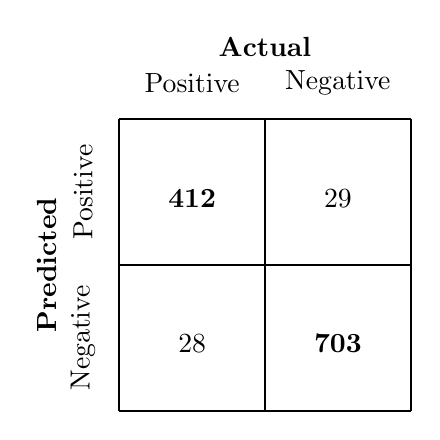
\begin{tikzpicture}[scale=1.85]
      \draw[thick] (0, 0) -- (2, 0);
      \draw[thick] (0, 0) -- (0, 2);
      \draw[thick] (2, 2) -- (2, 0);
      \draw[thick] (2, 2) -- (0, 2);
      \draw[thick] (0, 1) -- (2, 1);
      \draw[thick] (1, 0) -- (1, 2);
      \node[rotate=0] (h1) at (1, 2.5) {\textbf{Actual}};
        \node[rotate=0] (h11) at (0.5, 2.25) {Positive};
        \node[rotate=0] (h12) at (1.5, 2.25) {Negative};
      \node[rotate=90] (h2) at (-0.5, 1) {\textbf{Predicted}};
        \node[rotate=90] (h21) at (-0.25, 1.5) {Positive};
        \node[rotate=90] (h22) at (-0.25, 0.5) {Negative};
      \coordinate[label={\textbf{412}}] (TP) at (0.5, 1.33);
      \coordinate[label={ 28}] (FN) at (0.5, 0.33);
      \coordinate[label={ 29}] (FP) at (1.5, 1.33);
      \coordinate[label={\textbf{703}}] (TN) at (1.5, 0.33);
    \end{tikzpicture}
    \caption{Confusion matrix over the test set.}
    \label{figure:confusion}
  \end{figure}

  In random forests the features importance are calculated by averaging the features importance in each decision tree.
  For a decision tree the features importance are calculated during the fit and are computed as the normalized total reduction of the criterion brought by each feature. 

  The most important feature is PRF $\Delta\theta_{SQ}$ (\texttt{Pixel Response Function}), that basically is the angular offset on the plane of the sky between the centroid of the star and the calculated centroid of the star during the passage of the object of interest.
  It's very important because a lot of false positives are due to the transit of another star in binary systems.
  So, if this value is big it's most likely that the object of interest is not an exoplanet.
  For some reason, the planetary radius represents another discriminant feature to determinate if an hypothetical exoplanet is real or a false positive.
  It is possible that objects that have a very small radius can be attributed to measurements noise.

  In conclusion, we can say that most of the false positive occurrences are attributed to binary star systems and measurements noise.

  \begin{figure}
    \centering
    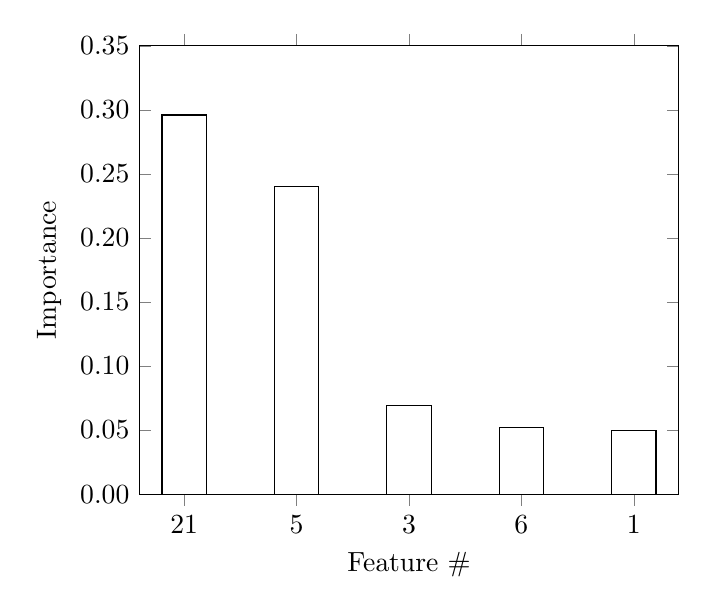
\begin{tikzpicture}
      \begin{axis}[
        ybar,
        ylabel=Importance,
        xlabel=Feature \#,
        symbolic x coords={21, 5, 3, 6, 1},
        bar width=16pt,
        ymin=0.0, ymax=0.35,
        ytick={0.0, 0.05, 0.10, 0.15, 0.20, 0.25, 0.30, 0.35},
        yticklabel style={/pgf/number format/fixed, /pgf/number format/fixed zerofill}
      ]
        \addplot[style={fill=white}] coordinates {
          (21, 0.296)
          (5, 0.24)
          (3, 0.069)
          (6, 0.052)
          (1, 0.050)
        };
      \end{axis}
    \end{tikzpicture}
    \caption{Five most important features importance.}
    \label{figure:importances}
  \end{figure}

\clearpage
\appendix
\appendixpage

\section{Exoplanet Selected Features}
  The documentation of the following exoplanet selected features can be found at \texttt{https://exoplanetarchive.ipac.caltech.edu}.
  However most of them are auto-explicative.
  The features used in this work are regarding the observed star, the processed features of the object of interest and various spectrometric metrics.
  \begin{multicols}{2}
    \label{appendix:features}
    \begin{enumerate}
      \item Orbital Period [$days$]
      \item Transit Duration [$hrs$]
      \item Transit Depth [$ppm$]
      \item Fitted Stellar Density [$g/cm^{3}$]
      \item Planetary Radius [$Earth\:radii$]
      \item Inclination [$deg$]
      \item Equilibrium Temperature [$K$]
      \item Insolation Flux [$Earth\:flux$]
      \item Stellar Effective Temperature [$K$]
      \item Stellar Surface Gravity [$\log_{10}(cm/s^{2})$]
      \item Stellar Metallicity [$dex$]
      \item Stellar Radius [$Solar\:radii$]
      \item Stellar Mass [$Solar\:mass$]
      \item RA [$decimal\:degrees$]
      \item Dec [$decimal\:degrees$]
      \item Kepler-band [$mag$]
      \item FW $\Delta\alpha$ [$sec$]
      \item FW $\Delta\delta$ [$arcsec$]
      \item PRF $\Delta\alpha_{SQ}$ [$arcsec$]
      \item PRF $\Delta\delta_{SQ}$ [$arcsec$]
      \item PRF $\Delta\theta_{SQ}$ [$arcsec$]
    \end{enumerate}
  \end{multicols}

\section{Decision tree split criterions}
  \label{appendix:splitcriterions}
  \subsection{Gini impurity}
    Citing \texttt{wikipedia.org}, Gini impurity is a measure of how often a randomly chosen element from the set would be incorrectly labeled if it was randomly labeled according to the distribution of labels in the subset.
    To compute Gini impurity for a set of items with $J$ classes, suppose $i\in\{1,2,...,J\}$, and let $p_{i}$ be the faction of items labeled with class $i$ in the set.
    \[{I} _{G}(p)=\sum _{i=1}^{J}p_{i}\sum _{k\neq i}p_{k}=\sum _{i=1}^{J}p_{i}(1-p_{i})=1-\sum _{i=1}^{J}{p_{i}}^{2}\]
  \subsection{Information gain}
    Information gain is based on the concept of entropy and information content from information theory.
    For each node of the tree, the information value represents the expected amount of information that would be needed to specify whether a new instance should be classified yes or no, given the example reached that node.
    Given $T$ the set of training examples and $X$ the selected feature.
    \[IG(T, X)=\mathrm{H}(T)-\mathrm{H}(T|X)=\mathrm{H}(T)-\sum_{x}{\Pr(X=x)\mathrm{H}(T|X=x)}\]

\bibliography{biblio.bib}
\bibliographystyle{unsrt}

\end{document}
